\documentclass[a4paper]{article}
\usepackage[
	pdftex,
	colorlinks=true,
	bookmarksnumbered=true,
	bookmarksopen=true,
	bookmarksopenlevel=3,
	pdfstartview=FitP,
	urlcolor=blue,
]{hyperref}
\pdfinfo{
	/Title(Esercitazione di Laboratorio: Misure su amplificatori)
	/Author(Coa Giulio, Licastro Dario, Montano Alessandra)
}
\usepackage[italian]{babel}
\usepackage{geometry,titling,mdsymbol,stmaryrd,graphicx,subcaption,amsmath}
\graphicspath{{./Image/}}
\renewcommand\maketitlehooka{
	\null
	\mbox{}
	\vfill
}
\renewcommand\maketitlehookd{
	\vfill
	\null
}
\title{
	\begin{center}
		Esercitazione di Laboratorio:
	\end{center}
	\newline
	\begin{center}
		Misure su amplificatori
	\end{center}
}
\author{
	Coa Giulio
	\and
	Licastro Dario
	\and
	Montano Alessandra
}
\begin{document}
	%-----------------------------------------------------------------------------
	%  TITLE
	%-----------------------------------------------------------------------------
	\begin{titlingpage}
		\maketitle
	\end{titlingpage}
	\newpage
	%-----------------------------------------------------------------------------
	%  PURPOSE OF THE EXPERIENCE
	%-----------------------------------------------------------------------------
	\section{Scopo dell'esperienza}
		Gli scopi di questa esercitazione sono:
		\begin{itemize}
			\item Analizzare il comportamento e misurare i parametri di moduli amplificatori (invertenti e non).
			\item Verificare alcune deviazioni rispetto al comportamento previsto con i modelli di prima approssimazione.
		\end{itemize}
	%-----------------------------------------------------------------------------
	%  INSTRUMENTATION USED
	%-----------------------------------------------------------------------------
	\section{Strumentazione utilizzata}
		La strumentazione usata durante l'esercitazione è:
		\begin{center}
			\begin{tabular}{ |c|c|c| }
				\hline
				\multirow{\textbf{Strumento}}	 & \textbf{Marca e Modello} & \textbf{Caratteristiche} \\
				\hline
				\multirow{Multimetro}			 & Agilent 34401A			& \\
				\multirow{Oscilloscopio}		 & Rigol DS1054Z			& 4 canali, \\
												 &							& $ B = 50 \, \mathrm{MHz} $, \\
												 &							& $ f_{\mathrm{c}} = 1 \, \mathrm{G\frac{Sa}{s}} $, \\
												 &							& $ R_{\mathrm{i}} = 1 \, \mathrm{M\Omega} $, \\
												 &							& $ C_{\mathrm{i}} = 13 \, \mathrm{pF} $, \\
												 &							& $ 12 \, \mathrm{Mbps} $ di profondità di memoria \\
				\multirow{Generatore di segnali} & Rigol DG1022				& 2 canali, \\
												 &							& $ f_{\mathrm{uscita}} = 20 \, \mathrm{MHz} $, \\
												 &							& $ Z_{\mathrm{uscita}} = 50 \, \mathrm{\Omega} $ \\
				\multirow{Alimentatore in DC}	 & Rigol DP832				& 3 canali \\
				\multirow{Sonda}				 & Rigol PVP215				& $ B = 35 \, \mathrm{MHz} $, \\
												 &							& $ V_{\mathrm{nominale}} = 300 \, \mathrm{V} $, \\
												 &							& $ L_{\mathrm{cavo}} = 1.2 \, \mathrm{m} $, \\
												 &							& $ R_{\mathrm{s}} = 1 \, \mathrm{M\Omega} $, \\
												 &							& Intervallo di compensazione: $ 10 \div 25 \, \mathrm{pF} $ \\
				\multirow{Scheda premontata}	 & A2						& \\
				\multirow{Cavi coassiali}		 &							& Capacità dell'ordine dei $ 80 \div 100 \, \mathrm{p\frac{F}{m}} $ \\
				\multirow{Connettori}			 &							& \\
				\hline
			\end{tabular}
		\end{center}
	%-----------------------------------------------------------------------------
	%  THEORETICAL PREMISES
	%-----------------------------------------------------------------------------
	\section{Premesse teoriche}
		\subsection{Incertezza sulla misura dell'oscilloscopio}
			La misura del valore di un segnale tramite l’oscilloscopio (sia esso l'ampiezza, la frequenza, il periodo, etc.) presenta un'incertezza che dipende, principalmente, da due fattori:
			\begin{itemize}
				\item l’incertezza strumentale introdotta dall’oscilloscopio (ricavabile dal manuale).
				\item l’incertezza di lettura dovuta all’errore del posizionamento dei cursori.
			\end{itemize}
			Quest’ultima incertezza deriva dal fatto che il segnale visualizzato non ha uno spessore nullo sullo schermo.
		\subsection{Amplificatore}
			Un amplificatore è un doppio bipolo unidirezionale caratterizzato dalla seguente relazione
			\begin{center}
				$ y(t) = A \cdot x(t) $
			\end{center}
			\newline
			Dove $ A $ è detto guadagno dell'amplifiatore.
			\begin{figure}[h!]
				\centering
				\begin{subfigure}{0.4\textwidth}
					\centering
					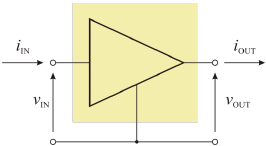
\includegraphics[scale=0.7]{amplificatore}
					\caption{Amplificatore.}
				\end{subfigure}
				\begin{subfigure}{0.4\textwidth}
					\centering
					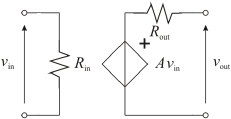
\includegraphics[scale=0.7]{amplificatoreCircuito}
					\caption{Circuito equivalente ad un amplificatore.}
				\end{subfigure}
				\label{fig:amplificatore}
			\end{figure}
			\newline
			In base al tipo di segnale in ingresso e in uscita, possiamo distinguere quattro tipi di amplifiatori:
			\begin{itemize}
				\item Amplificatore di Tensione.
				\item Amplificatore di Transconduttanza.
				\item Amplificatore di Transresistenza.
				\item Amplificatore di Corrente.
			\end{itemize}
			\subsubsection{Amplificatore operazionale}
				L'amplificatore operazionale è un amplificatore differenziale, ovvero amplifica la differenza delle tensioni ai suoi capi, che presenta un'amplificazione $ A_{\mathrm{d}} $ idealmente infinita.
				\begin{equation*}
					\begin{split}
						A_{\mathrm{d}} &= \frac{v_{\mathrm{out}}}{v_{\mathrm{d}}} = \\
									   &= \frac{v_{\mathrm{out}}}{v^{+} - v^{-}}
					\end{split}
				\end{equation*}
				\begin{figure}[h!]
					\centering
					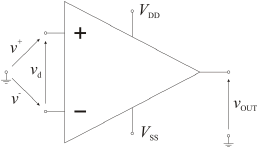
\includegraphics[scale=0.7]{amplificatoreOperazionale}
					\caption{Amplificatore operazionale}
					\label{fig:amplificatoreOperazionale}
				\end{figure}
				\subsubsection{Amplificatore invertente}
					L'amplificatore invertente è un derivato dell'amplificatore di transresistenza che fornisce, in uscita, un segnale proporzionale al segnale in ingresso ma che presenta fase invertita rispetto ad esso; esso caratterizzato dalle seguenti relazioni
					\begin{equation*}
						\begin{split}
							v_{\mathrm{out}} &= A_{\mathrm{v}} \cdot v_{\mathrm{in}} = \\
											 &= -\frac{R_{2}}{R_{1}} \cdot v_{\mathrm{in}}
						\end{split}
					\end{equation*}
					\begin{center}
						$ R_{\mathrm{in}} = R_{1} $
					\end{center}
					\newline
					\begin{center}
						$ R_{\mathrm{out}} = 0 $
					\end{center}
					\newline
					\begin{figure}[h!]
						\centering
						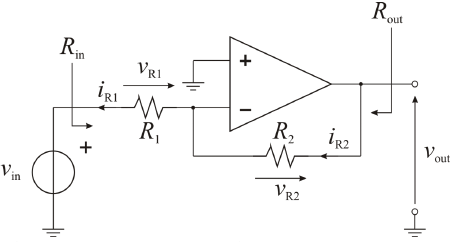
\includegraphics[scale=0.7]{amplificatoreInvertente}
						\caption{Amplificatore invertente}
						\label{fig:amplificatoreInvertente}
					\end{figure}
					\newline
					\begin{scriptsize}
						\textbf{N.B.} $ R_{\mathrm{in}} $ non è necessariamente elevata. 
					\end{scriptsize}
	%-----------------------------------------------------------------------------
	%  LABORATORY EXPERIENCE
	%-----------------------------------------------------------------------------
	\section{Esperienza in laboratorio}
		Abbiamo realizzato il circuito richiesto, collegando:
		\begin{itemize}
			\item Il generatore di segnali al connettore coassiale J1.
			\item L'alimentatore duale viene connesso, in modalità tracking, al morsetto J8.
			\item L'oscilloscopio, tramite due cavi coassiali BNC-coccodrillo, all'ingresso e all'uscita del circuito, rispettivamente gli ancoraggi J4 e J5 (massa) e J6 e J7 (massa).
		\end{itemize}
		E portando gli switch S1 ed S2, che determinano il tipo d'amplificatore da usare, se invertente o meno, sull'1, ovvero selezionando l'amplificatore non-invertente.
		\subsection{Parametri di un amplificatore}
			\subsubsection{Misura del guadagno}
				Abbiamo disposto la scheda premontata in modo da applicare la tensione del generatore direttamente all'ingresso dell'amplificatore non-invertente, seguendo la seguente tabella
				\begin{center}
					\begin{tabular}{ |c|c|c| }
						\hline
						\multirow{\textbf{Interruttore}} & \textbf{Posizione} & \textbf{Note} \\
						\hline
						\multirow{S1}		     		 & 2				  & \\
						\multirow{S2}		     		 & 2				  & \\
						\multirow{S3}		     		 & 2				  & chiuso \\
						\multirow{S4}		     		 & 2				  & chiuso \\
						\multirow{S5}		     		 & 2				  & chiuso \\
						\multirow{S6}		     		 & 1				  & aperto \\
						\multirow{S7}		     		 & 1				  & aperto \\
						\multirow{S8}		     		 & 1				  & aperto \\
						\multirow{S9}		     		 & 1				  & aperto \\
						\hline
					\end{tabular}
				\end{center}
				Impostando il generatore di segnali come richiesto, abbiamo misurato, tramite cursori, l'ampiezza d'ingresso e d'uscita al fine di calcolare il guadagno dell'amplificatore.
			\subsubsection{Misura della resistenza equivalente in ingresso}
				Al fine di misurare la resistenza in ingresso all'amplificatore, ci avvaliamo di una resistenza esterna, di valore noto, mettendola in serie al generatore; in questo modo si va a creare un partitore di tensione che sfrutteremo per determinare $ R_{\mathrm{i}} $.
				\newline
				Nel concreto, ciò avviene commutando la posizione dello switch S5, che determina la presenza della resistenza $ R_{9} $ nel circuito.
				\newline
				Abbiamo effettuato le misurazioni sulla tensione di uscita, poichè ciò permette di evidenziare maggiormente quanto la resistenza influenzi il segnale.
			\subsubsection{Misura della resistenza equivalente di uscita}	
				Al fine di misurare la resistenza di uscita all'amplificatore, ci avvaliamo di una resistenza esterna, di valore noto, mettendola in serie all'uscita; in questo modo si va a creare un partitore di tensione che sfrutteremo per determinare $ R_{\mathrm{u}} $.
				\newline
				Nel concreto, ciò viene ottenuto commutando la posizione dello switch S6, che determina la presenza della resistenza $ R_{10} $ nel circuito.
				\newline
				Abbiamo effettuato le misurazioni sulla tensione di uscita, poichè ciò permette di evidenziare maggiormente quanto la resistenza influenzi il segnale.				
				\newline
				\begin{scriptsize}
					\textbf{N.B.} Ovviamente, prima di procedere con questa parte dell'esercitazione, abbiamo ripristinato lo stato iniziale dell'amplificatore, ovvero abbiamo cortocircuitato la resistenza $ R_{9} $. 
				\end{scriptsize}
		\subsection{Risposta in frequenza di un amplificatore con celle RC esterne}
			Abbiamo disposto la scheda premontata come richiesto, seguendo la seguente tabella
			\begin{center}
				\begin{tabular}{ |c|c|c| }
					\hline
					\multirow{\textbf{Interruttore}} & \textbf{Posizione} & \textbf{Note} \\
					\hline
					\multirow{S1}		     		 & 2				  & \\
					\multirow{S2}		     		 & 2				  & \\
					\multirow{S3}		     		 & 2				  & $ C_{10} $ inserito \\
					\multirow{S4}		     		 & 1				  & $ C_{5} $ non cortocircuitato \\
					\multirow{S5}		     		 & 2				  & chiuso \\
					\multirow{S6}		     		 & 1				  & aperto \\
					\multirow{S7}		     		 & 1				  & aperto \\
					\multirow{S8}		     		 & 2				  & $ C_{6} $ inserito \\
					\multirow{S9}		     		 & 1				  & $ C_{9} $ non inserito \\
					\hline
				\end{tabular}
			\end{center}
			Successivamente, abbiamo eseguito le misure di guadagno per frequenze da $ 300 \, \mathrm{Hz} $ a $ 1 \, \mathrm{MHz} $, con due misure per decade, usando, come consigliatoci, un segnale con ampiezza $ V_{\mathrm{pp}} $ pari a $ 1 \, \mathrm{V} $ per frequenze fino a $ 30 \, \mathrm{kHz} $ ed un segnale con ampiezza $ V_{\mathrm{pp}} $ pari a $ 200 \, \mathrm{mV} $ per frequenze a partire da $ 100 \, \mathrm{kHz} $.
		\subsection{Amplificatore invertente}
			Abbiamo disposto la scheda premontata di modo da utizzare l'amplificatore invertente, ovvero abbiamo commutato gli switch S1 ed S2, e, successivamente, abbiamo ripetuto l'esperienza effettuata precedentemente e verificato l'inversione di fase tra il segnale e la tensione in uscita.
	%-----------------------------------------------------------------------------
	%  RESULTS
	%-----------------------------------------------------------------------------
	\section{Risultati}
		\subsection{Parametri di un amplificatore}
			\subsubsection{Misura del guadagno}
				\begin{center}
					\begin{tabular}{ |c|c|c|c| }
						\hline
						\multirow{\textbf{$ V_{\mathrm{i}} $ [$ \mathrm{V} $]}} & \textbf{$ V_{\mathrm{u}} $ [$ \mathrm{V} $]} & \textbf{$ A_{\mathrm{v}} $} & \textbf{$ A_{\mathrm{v}} $ [$ \mathrm{dB} $]} \\
						\hline
						\multirow{$ 1.12 $}		     		    				& $ 8.72 $									   & $ 7.78 $					 & $ 17.82 $ \\
						\hline
					\end{tabular}
				\end{center}
				Come si può vedere, il risultato ottenuto rientra nel range fornito dal costruttore ($ 9.33 \pm 0.93 $).
				\begin{figure}[h!]
					\centering
					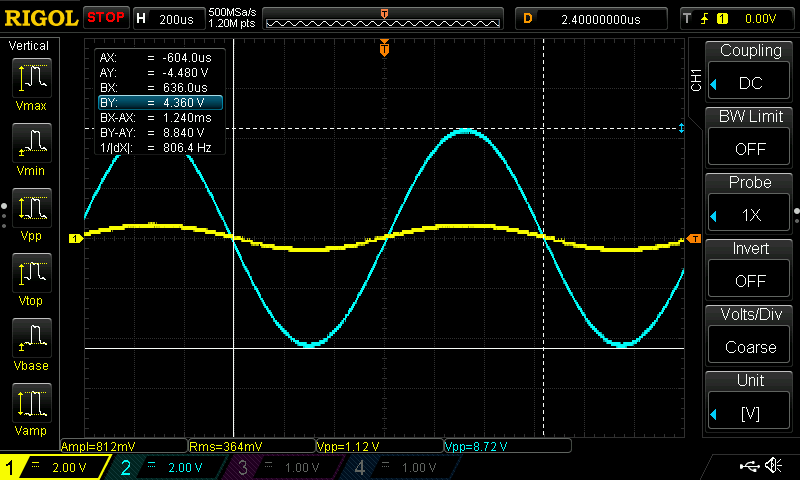
\includegraphics[scale=0.3]{misuraDelGuadagnoAmplificatoreNonInvertente}
					\caption{Misura del guadagno dell'amplificatore non-invertente.}
					\label{fig:misuraDelGuadagnoAmplificatoreNonInvertente}
				\end{figure}
			\subsubsection{Misura della resistenza equivalente in ingresso}
				\begin{center}
					\begin{tabular}{ |c|c| }
						\hline
						\multirow{} 						 & \textbf{$ V_{\mathrm{u}} $ [$ \mathrm{V} $]} \\
						\hline
						\multirow{$ R_{9} $ inserita}		 & $ 4.64 \pm 0.48 $ \\
						\multirow{$ R_{9} $ cortocircuitata} & $ 8.72 \pm 0.48 $ \\
						\hline
					\end{tabular}
				\end{center}
				Sfruttando il partitore di tensione formatosi all'ingresso dell'amplifiatore quando la resistenza $ R_{9} $ è inserita, possiamo scrivere
				\begin{equation*}
					\begin{split}
						w &= \frac{v_{\mathrm{out,R_{9}}}}{v_{\mathrm{out}}} = \\
						  &= \frac{A_{\mathrm{v}} \cdot V_{\mathrm{i,R_{9}}}}{A_{\mathrm{v}} \cdot V_{\mathrm{i}}} = \\
						  &= \frac{V_{\mathrm{i,R_{9}}}}{V_{\mathrm{i}}} = \\
						  &= \frac{v_{\mathrm{s}} \cdot \frac{R_{\mathrm{i}}}{R_{9} + R_{\mathrm{i}}}}{v_{\mathrm{s}}} = \\
						  &= \frac{R_{\mathrm{i}}}{R_{9} + R_{\mathrm{i}}} = \\
						  &= 532m
					\end{split}
				\end{equation*}
				Da cui
				\begin{equation*}
					\begin{split}
						R_{\mathrm{i}} &= w \cdot R_{9} \cdot \frac{1}{1 - w} = \\
									   &= 532m \cdot 10k \cdot \frac{1}{1 - 532m} = \\
									   &= 11.4 \, \mathrm{k\Omega}
					\end{split}
				\end{equation*}
				Il valore ottenuto non rientra nel range dato dal costruttore ($ 10 \pm 0.5 \, \mathrm{k\Omega} $) a causa dei vari contributi d'incertezza dati dagli strumenti.
				\begin{figure}[h!]
					\centering
					\begin{subfigure}{0.4\textwidth}
						\centering
						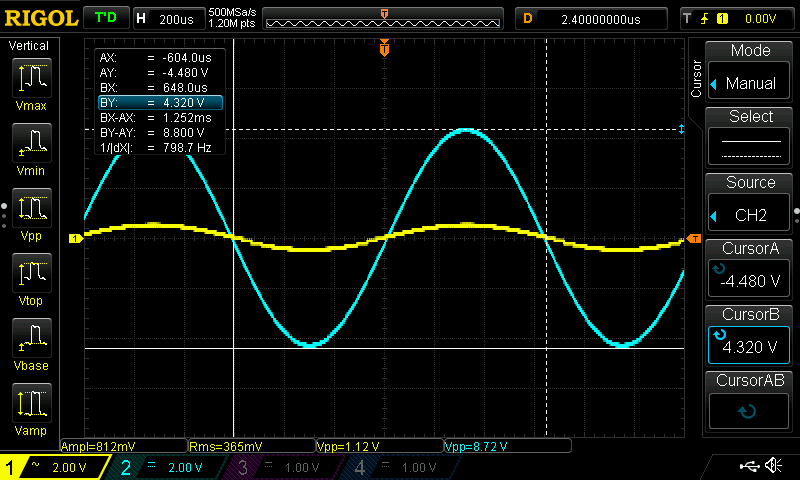
\includegraphics[scale=0.2]{misuraDellaResistenzaEquivalenteInIngressoAmplificatoreNonInvertenteR9InCorto}
						\caption{Misura della resistenza equivalente d'ingresso con R9 cortocircuitata.}
					\end{subfigure}
					\begin{subfigure}{0.4\textwidth}
						\centering
						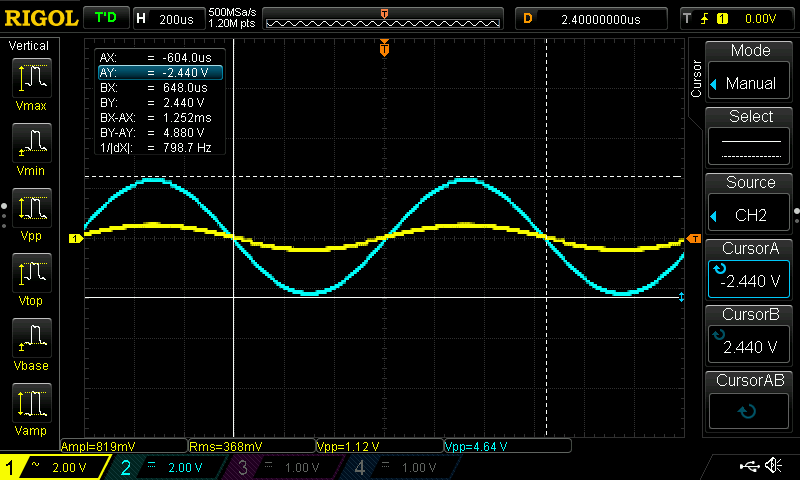
\includegraphics[scale=0.2]{misuraDellaResistenzaEquivalenteInIngressoAmplificatoreNonInvertenteR9Inserita}
						\caption{Misura della resistenza equivalente d'ingresso con R9 inserita.}
					\end{subfigure}
					\label{fig:misuraDellaResistenzaEquivalenteInIngressoAmplificatoreNonInvertente}
				\end{figure}
			\subsubsection{Misura della resistenza equivalente di uscita}	
				\begin{center}
					\begin{tabular}{ |c|c| }
						\hline
						\multirow{} 						  & \textbf{$ V_{\mathrm{u}} $ [$ \mathrm{V} $]} \\
						\hline
						\multirow{$ R_{10} $ inserita}		  & $ 4.40 $ \\
						\multirow{$ R_{10} $ cortocircuitata} & $ 8.72 $ \\
						\hline
					\end{tabular}
				\end{center}
				Sfruttando il partitore di tensione formatosi all'uscita dell'amplifiatore quando la resistenza $ R_{10} $ è inserita, possiamo scrivere
				\begin{equation*}
					\begin{split}
						w &= \frac{v_{\mathrm{out,R_{10}}}}{v_{\mathrm{out}}} = \\
						  &= \frac{A_{\mathrm{v}} \cdot V_{\mathrm{i,R_{10}}}}{A_{\mathrm{v}} \cdot V_{\mathrm{i}}} = \\
						  &= \frac{V_{\mathrm{i,R_{10}}}}{V_{\mathrm{i}}} = \\
						  &= \frac{v_{\mathrm{s}} \cdot \frac{R_{\mathrm{u}}}{R_{10} + R_{\mathrm{u}}}}{v_{\mathrm{s}}} = \\
						  &= \frac{R_{\mathrm{u}}}{R_{10} + R_{\mathrm{u}}} = \\
						  &= 505m
					\end{split}
				\end{equation*}
				Da cui
				\begin{equation*}
					\begin{split}
						R_{\mathrm{u}} &= w \cdot R_{10} \cdot \frac{1}{1 - w} = \\
									   &= 505m \cdot 1k \cdot \frac{1}{1 - 505m} = \\
									   &= 1.02 \, \mathrm{k\Omega}
					\end{split}
				\end{equation*}
				Il valore ottenuto rientra nel range dato dal costruttore ($ 1 \pm 0.05 \, \mathrm{k\Omega} $).
				\begin{figure}[h!]
					\centering
					\begin{subfigure}{0.4\textwidth}
						\centering
						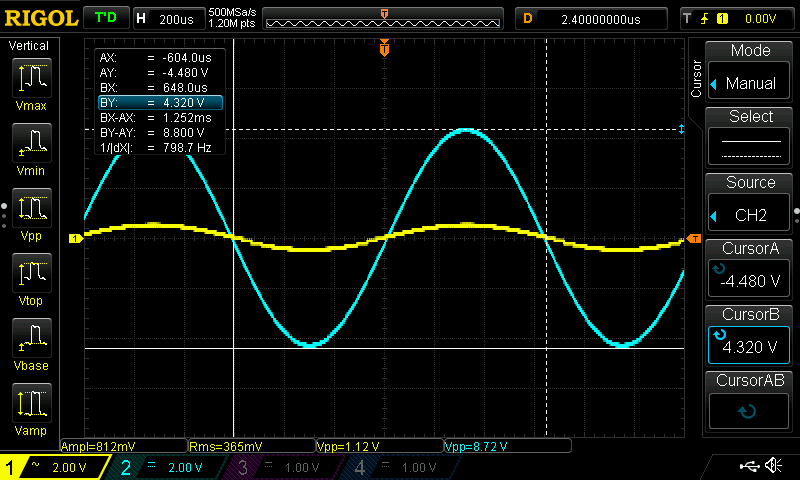
\includegraphics[scale=0.2]{misuraDellaResistenzaEquivalenteInIngressoAmplificatoreNonInvertenteR9InCorto}
						\caption{Misura della resistenza equivalente d'uscita con R10 cortocircuitata.}
					\end{subfigure}
					\begin{subfigure}{0.4\textwidth}
						\centering
						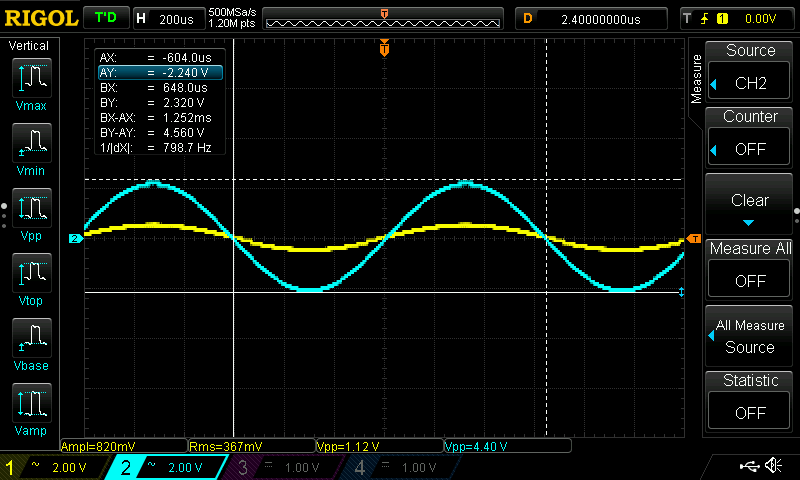
\includegraphics[scale=0.2]{misuraDellaResistenzaEquivalenteDiUscitaAmplificatoreNonInvertenteR10Inserita}
						\caption{Misura della resistenza equivalente d'uscita con R10 inserita.}
					\end{subfigure}
					\label{fig:misuraDellaResistenzaEquivalenteDiUscitaAmplificatoreNonInvertente}
				\end{figure}
		\subsection{Risposta in frequenza di un amplificatore con celle RC esterne}
			\begin{center}
				\begin{tabular}{ |c|c|c|c| }
					\hline
					\multirow{\textbf{Frequenza}} & \textbf{Pulsazione} & \textbf{$ A_{\mathrm{v}} $ calcolato [$ \mathrm{dB} $]} & \textbf{$ A_{\mathrm{v}} $ misurato [$ \mathrm{dB} $]} \\
					\hline
					\multirow{$ 300 \, \mathrm{Hz} $}  & $ 1.88 \, \mathrm{k\frac{rad}{s}} $ & $ 103 $ & $ 13.1 $ \\
					\multirow{$ 1 \, \mathrm{kHz} $}   & $ 6.28 \, \mathrm{k\frac{rad}{s}} $ & $ 103 $ & $ 14.1 $ \\
					\multirow{$ 3 \, \mathrm{kHz} $}   & $ 18.8 \, \mathrm{k\frac{rad}{s}} $ & $ 103 $ & $ 17.1 $ \\
					\multirow{$ 10 \, \mathrm{kHz} $}  & $ 62.8 \, \mathrm{k\frac{rad}{s}} $ & $ 103 $ & $ 16.5 $ \\
					\multirow{$ 30 \, \mathrm{kHz} $}  & $ 188 \, \mathrm{k\frac{rad}{s}} $  & $ 103 $ & $ 11.7 $ \\
					\multirow{$ 100 \, \mathrm{kHz} $} & $ 628 \, \mathrm{k\frac{rad}{s}} $  & $ 103 $ & $ 3.29 $ \\
					\multirow{$ 300 \, \mathrm{kHz} $} & $ 1.88 \, \mathrm{M\frac{rad}{s}} $ & $ 103 $ & $ -8.89 $ \\
					\multirow{$ 1 \, \mathrm{MHz} $}   & $ 6.28 \, \mathrm{M\frac{rad}{s}} $ & $ 103 $ & $ -23.4 $ \\
					\hline
				\end{tabular}
			\end{center}
			% foto Bode
		\subsection{Amplificatore invertente}
			\subsubsection{Misura del guadagno}
				\begin{center}
					\begin{tabular}{ |c|c|c|c| }
						\hline
						\multirow{\textbf{$ V_{\mathrm{i}} $ [$ \mathrm{V} $]}} & \textbf{$ V_{\mathrm{u}} $ [$ \mathrm{V} $]} & \textbf{$ A_{\mathrm{v}} $} & \textbf{$ A_{\mathrm{v}} $ [$ \mathrm{dB} $]} \\
						\hline
						\multirow{$ 1.12 $}		     		    				& $ 10.3 $									   & $ 9.20 $					 & $ 19.27 $ \\
						\hline
					\end{tabular}
				\end{center}
				Come si può vedere, il risultato ottenuto rientra nel range fornito dal costruttore ($ 9.33 \pm 0.93 $).
				\newline
				Alla frequenza $ f = 1 \, \mathrm{kHz} $, il guadagno dell'amplificatore invertente è pari a
				\begin{center}
					\begin{tabular}{ |c|c|c|c| }
						\hline
						\multirow{\textbf{$ V_{\mathrm{i}} $ [$ \mathrm{V} $]}} & \textbf{$ V_{\mathrm{u}} $ [$ \mathrm{V} $]} & \textbf{$ A_{\mathrm{v}} $} & \textbf{$ A_{\mathrm{v}} $ [$ \mathrm{dB} $]} \\
						\hline
						\multirow{$ 1.08 $}		     		    				& $ 10.3 $									   & $ 9.54 $					 & $ 19.59 $ \\
						\hline
					\end{tabular}
				\end{center}
				\begin{figure}[h!]
					\centering
					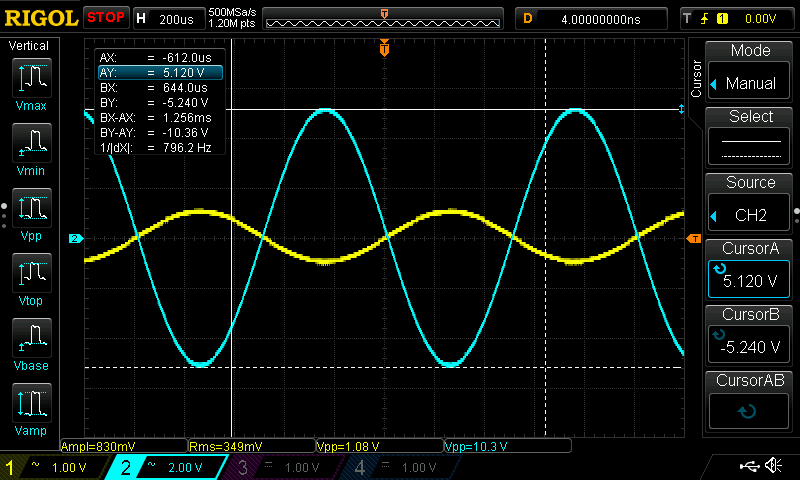
\includegraphics[scale=0.3]{misuraDelGuadagnoAd1kAmplificatoreInvertente}
					\caption{Misura del guadagno dell'amplificatore invertente alla frequenza $ f = 1 \, \mathrm{kHz} $.}
					\label{fig:misuraDelGuadagnoAd1kAmplificatoreInvertente}
				\end{figure}
				\newline
			\subsubsection{Misura della resistenza equivalente in ingresso}
				\begin{center}
					\begin{tabular}{ |c|c| }
						\hline
						\multirow{} 						 & \textbf{$ V_{\mathrm{u}} $ [$ \mathrm{V} $]} \\
						\hline
						\multirow{$ R_{9} $ inserita}		 & $ 6.24 $ \\
						\multirow{$ R_{9} $ cortocircuitata} & $ 10.3 $ \\
						\hline
					\end{tabular}
				\end{center}
				Sfruttando il partitore di tensione formatosi all'ingresso dell'amplifiatore quando la resistenza $ R_{9} $ è inserita, possiamo scrivere
				\begin{equation*}
					\begin{split}
						w &= \frac{v_{\mathrm{out,R_{9}}}}{v_{\mathrm{out}}} = \\
						  &= \frac{A_{\mathrm{v}} \cdot V_{\mathrm{i,R_{9}}}}{A_{\mathrm{v}} \cdot V_{\mathrm{i}}} = \\
						  &= \frac{V_{\mathrm{i,R_{9}}}}{V_{\mathrm{i}}} = \\
						  &= \frac{v_{\mathrm{s}} \cdot \frac{R_{\mathrm{i}}}{R_{9} + R_{\mathrm{i}}}}{v_{\mathrm{s}}} = \\
						  &= \frac{R_{\mathrm{i}}}{R_{9} + R_{\mathrm{i}}} = \\
						  &= 606m
					\end{split}
				\end{equation*}
				Da cui
				\begin{equation*}
					\begin{split}
						R_{\mathrm{i}} &= w \cdot R_{9} \cdot \frac{1}{1 - w} = \\
									   &= 606m \cdot 10k \cdot \frac{1}{1 - 606m} = \\
									   &= 15.4 \, \mathrm{k\Omega}
					\end{split}
				\end{equation*}
				Il valore ottenuto rientra nel range dato dal costruttore ($ 15 \pm 0.75 \, \mathrm{k\Omega} $).
				\begin{figure}[h!]
					\centering
					\begin{subfigure}{0.4\textwidth}
						\centering
						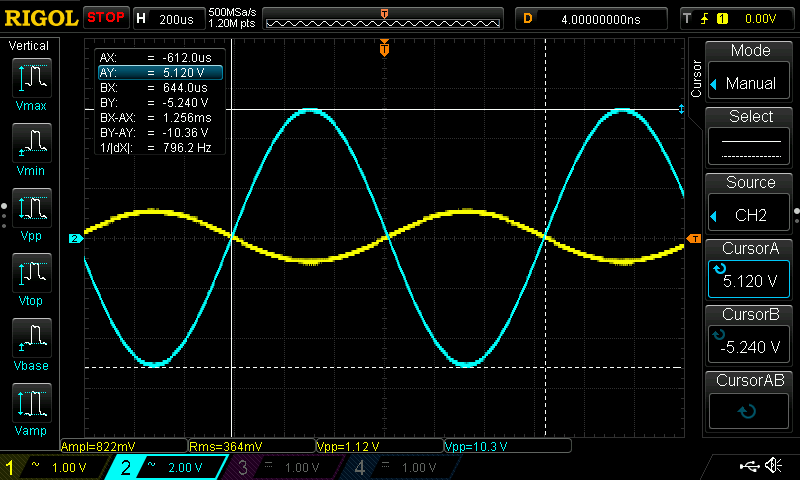
\includegraphics[scale=0.2]{misuraDellaResistenzaEquivalenteInIngressoAmplificatoreInvertenteR9InCorto}
						\caption{Misura della resistenza equivalente d'ingresso con R9 cortocircuitata.}
					\end{subfigure}
					\begin{subfigure}{0.4\textwidth}
						\centering
						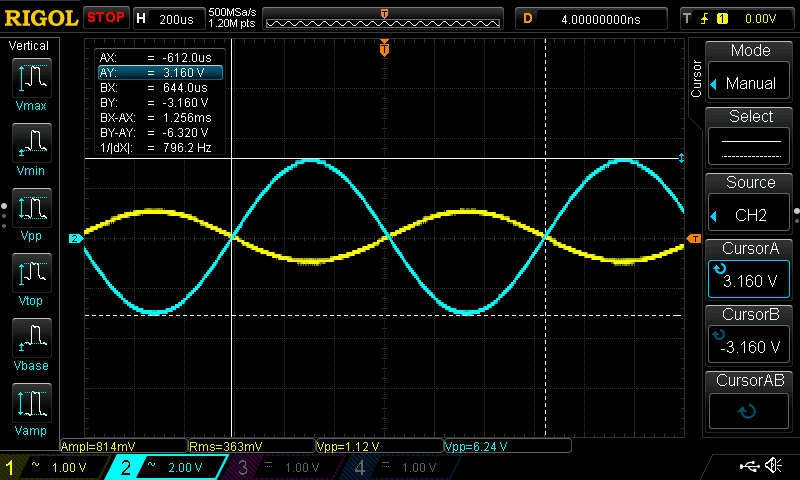
\includegraphics[scale=0.2]{misuraDellaResistenzaEquivalenteInIngressoAmplificatoreInvertenteR9Inserita}
						\caption{Misura della resistenza equivalente d'ingresso con R9 inserita.}
					\end{subfigure}
					\label{fig:misuraDellaResistenzaEquivalenteInIngressoAmplificatoreInvertente}
				\end{figure}
			\subsubsection{Misura della resistenza equivalente di uscita}	
				\begin{center}
					\begin{tabular}{ |c|c| }
						\hline
						\multirow{} 				   		  & \textbf{$ V_{\mathrm{u}} $ [$ \mathrm{V} $]} \\
						\hline
						\multirow{$ R_{10} $ inserita} 		  & $ 10.3 $ \\
						\multirow{$ R_{10} $ cortocircuitata} & $ 10.3 $ \\
						\hline
					\end{tabular}
				\end{center}
				Dato che le due tensioni misurate sono uguali, deduciamo che il valore di $ R_{\mathrm{u}} $ è trascurabile e, quindi, essa è assimilabile ad un cortocircuito.
				\begin{figure}[h!]
					\centering
					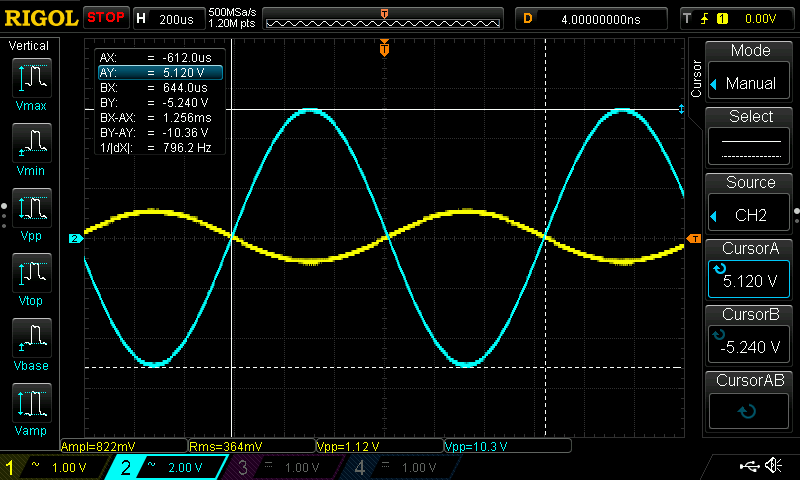
\includegraphics[scale=0.2]{misuraDellaResistenzaEquivalenteInIngressoAmplificatoreInvertenteR9InCorto}
					\caption{Misura della resistenza equivalente d'uscita.}
					\label{fig:misuraDellaResistenzaEquivalenteDiUscitaAmplificatoreInvertente}
				\end{figure}
\end{document}